% CHAPTER 3
\chapter{MATERIALS AND METHODS}
\label{chp:chapter3}

\section{Mapping RBP binding sites}
To map the binding sites of RBPs, we downloaded 103 position frequency matrices (PFMs) that correspond to 85 human RBPs from the RNAcompete paper \cite{rnacompete_13}. These PFMs (which are of length seven or eight) are generated from the alignment of top 10 7-mers determined using all data (i.e. both setA and setB of RNAcompete pool). Rather than using these top 10 7-mers directly, we generated the top 10 n-mers from these PFMs. In this way, we also represented motifs that are longer than seven. In addition to RNAcompete motifs, we downloaded the motifs (consensus motifs and the top 10 n-mer when a PFM is available) for the following well-known RBPs from RBPDB database \cite{rbpdb_11}: HNRNPAB, PUM1, PUM2, ELAVL2, KHSRP, ZFP36, AUF1 and CUGBP. 

We downloaded human 3'UTRs from UCSC Genome Browser (on February 16th, 2014) and determined the genome-wide binding sites of each RBP by finding matches to its top 10 n-mers or consensus motifs on human 3'UTR sequences. We downloaded CLIP-seq and PARCLIP data for a list of RBPs (HuR, FMR1, FUS, FXR1, FXR2, HNRNPA1, HNRNPA2B1, HNRNPC, IGF2BP1-3, LIN28, PUM2, QKI, SRSF1, TDP-43, TIA1, TIAL1) from doRINA database \cite{dorina_11}. In addition to these RBP specific CLIP datasets, we downloaded gPARCLIP-determined peaks \cite{baltz_12}. gPARCLIP dataset contains genome-wide protein-occupied regions bound by any RBP in HEK293T cells. However, the identity of a particular RBP that binds to a region is unknown. 

We first intersected the peaks identified with CLIP or gPARCLIP  with human 3'UTRs. To correct for the background binding bias in CLIP-based techniques as identified by Friedersdorf et al. \cite{friedersdorf_14}, we excluded parts of peaks that overlap with regions that correspond to background binding. In summary, for each putative RBP site we keep track of the following information: (i) the start and end position; (ii) a flag showing whether the site is located in a CLIP- or gPARCLIP-determined peak; and (iii) conservation score calculated as the average PhastCons score \cite{siepel_05} (phastCons100way track downloaded from UCSC Genome Browser) across the motif (Figure \ref{overview}).

\clearpage

\section{Mapping miRNA binding sites}
To determine miRNA binding sites, we downloaded the target sites predicted by TargetScan and PicTar methods \cite{targetscan_05, pictar_05}. We downloaded AGO1-4 PARCLIP, AGO2 CLIP-seq and AGO2-MNase PARCLIP datasets from doRINA database, and removed background binding bias as described in the previous section. We also downloaded experimentally verified miRNA targets from miRTarBase database \cite{mirtarbase}. The interactions in miRTarBase database specify only whether a miRNA interacts with an mRNA without providing the exact position of the target site on the mRNA. Therefore, we assumed that a target miRNA site on an mRNA is supported by miRTarBase if that miRNA-mRNA interaction exists in the database. For each putative miRNA binding site, we keep track of its start and end position, a flag showing whether the site is supported by TargetScan, PicTar or both, a flag showing whether it is supported by miRTarBase and a flag whether the site is located in CLIP- or PARCLIP-determined peaks (Figure \ref{overview}).

\section{Compilation of datasets related to post-transcriptional regulation}

The following datasets were downloaded from the supplementary material of the corresponding papers:
\begin{itemize}
\item \textbf{Knockdown datasets:} Log fold changes (LFCs) of transcript abundance upon HuR knockdown in  HEK293 and HeLa cells from \cite{mukharjee_11} and \cite{lebedeva_11}, respectively. 
\item \textbf{Zhao dataset:} The effect of human 3'UTR segments (160-nts long) to mRNA stability and steady-state mRNA abundance in BEAS-2B human bronchial epithelial cells \cite{zhao_14}.
\item \textbf{Schueler dataset:} mRNA half-lives measured in HEK293 and MCF7 cells \cite{schueler_14}. Average of the two replicate measurements is used. 
\end{itemize}

\clearpage
%\shorthandoff{=}
\begin{figure}[H]
   \centering
   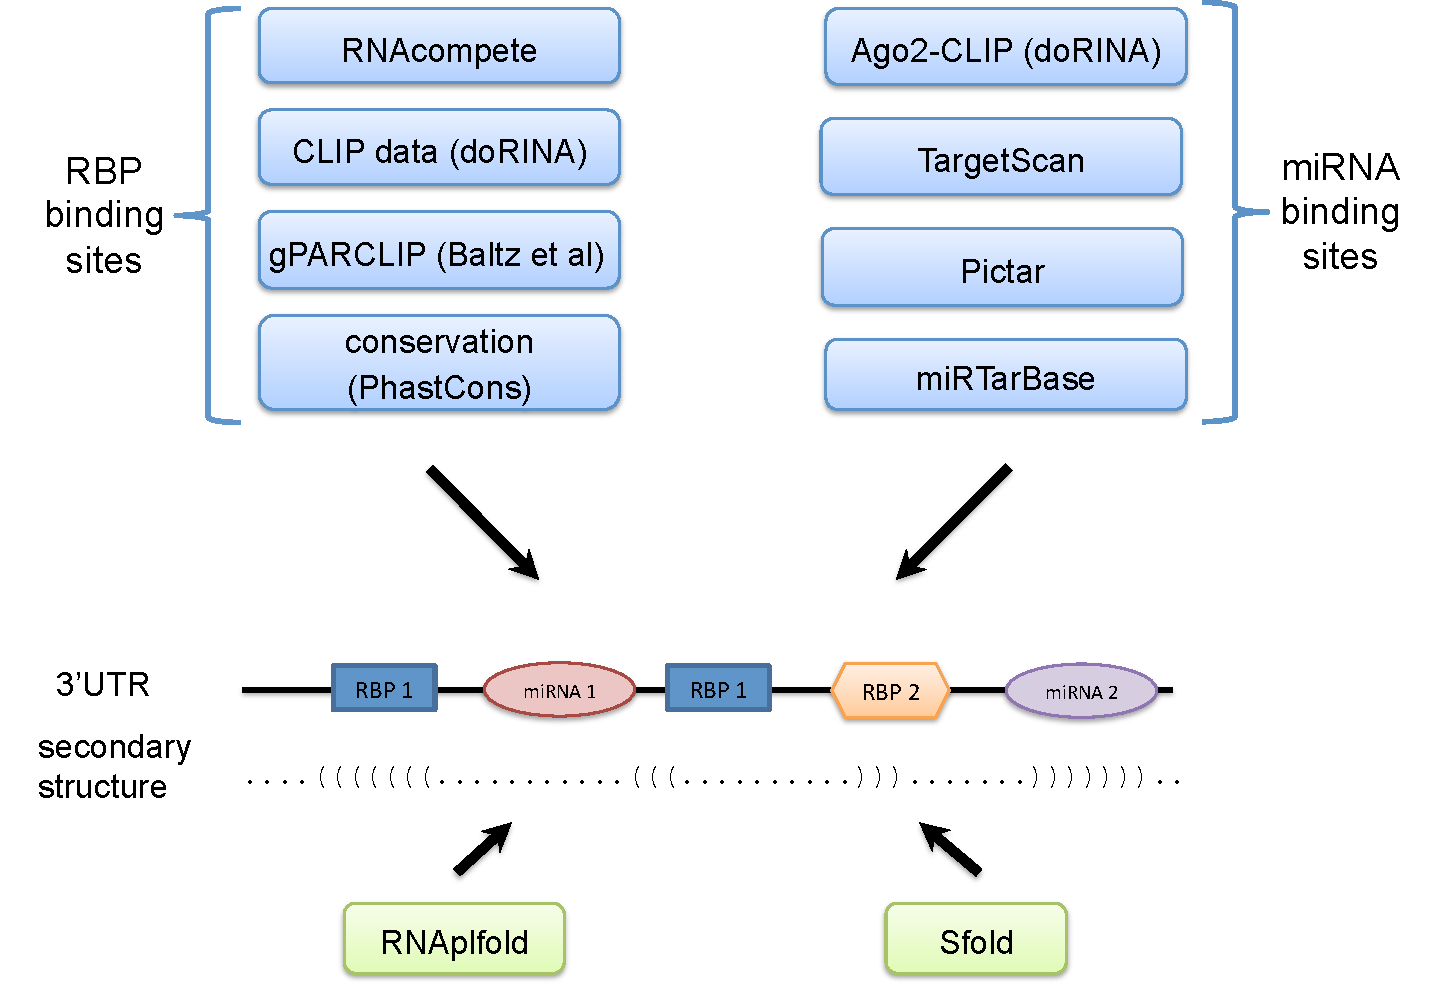
\includegraphics[width=0.7\textwidth]{ch3_materials_methods/figures/Figure1}

\caption[]{Mapping of RBP and miRNA binding sites on human 3'UTRs. RBP binding sites are mapped by leveraging RNAcompete PFMs, CLIP- and PARCLIP-determined peaks and PhastCons conservation scores. miRNA binding sites are mapped by combining TargetScan and PicTar predictions with Ago-CLIP datasets and experimentally-verified interactions in miRTarBase database. Also, the secondary structure of the 3'UTRs are predicted with RNAplfold and Sfold. In particular, accessibility of a site is calculated by RNAplfold, and the probability of a site to form a stem-loop by binding to another site is calculated by Sfold.}
\label{overview}
\end{figure}
%\shorthandon{=}


The set of expressed RBPs and miRNAs vary widely between different cell lines. As such, it is important to consider only those factors that are expressed in the corresponding cell line in the analysis of  the datasets above. We used the following sources to define the set of expressed RBPs and miRNAs in a given cell type:
\begin{itemize}
\item HEK293 cells: 
\begin{itemize}
\item RBPs: quantitative mass spectrometry results  \cite{baltz_12}.
\item miRNAs: top 100 expressed miRNAs identified with small-RNA sequencing \cite{hafner_10}.
\end{itemize}
\item HeLa cells:
\begin{itemize}
\item RBPs: immunohistochemistry results from Human Protein Atlas database \cite{proteinatlas}.
\item miRNAs: top 100 expressed miRNAs identified with small-RNA sequencing \cite{lebedeva_11}.
\end{itemize}
\item MCF7 cells:
\begin{itemize}
\item RBPs: immunohistochemistry results from Human Protein Atlas database.
\item miRNAs: top 100 expressed miRNAs identified with small-RNA sequencing \cite{anbalagan_14}.
\end{itemize}
\item BEAS-2B cells:
\begin{itemize}
\item RBPs: immunohistochemistry results from Human Protein Atlas database.
\item miRNAs:  top 100 expressed miRNAs identified with small-RNA sequencing \cite{zhao_14}.
\end{itemize}
\end{itemize}

For datasets that contain measurements mapped to gene IDs other than human RefSeq transcript IDs, we used the Synergizer tool for ID conversion \cite{synergizer}. 

We also checked the overlap in the set of expressed RBPs across the cell lines. Tables \ref{tbl:expressed_rbps} and \ref{tbl:expressed_mirnas} show the number of expressed RBPs and miRNAs in each cell line along with the percent overlap of expressed RBPs in different cell lines.
\hfill

\begin{table}[H]
\caption[Number of expressed RBPs in each cell line]{The numbers within parenthesis correspond to the total number of RBPs expressed in that cell line. Besides, percent of overlapping expressed RBPs between each pair of cell lines are shown. For example, \%95.65 of expressed RBPs in HEK293 cells are also expressed in HeLa cells. On the other hand, \%80.73 of expressed RBPs in HeLa cells are also expressed in HEK293 cells.}
\begin{tabular*}{\textwidth}{l @{\extracolsep{\fill}} c c c c}
%\rowcolor{LightCyan}
Cell types &  HEK293 (92) & HeLa (109) & BEAS2B (97) & MCF7 (102) \\ [0.5ex]
\hline\hline
HEK293 (92) & \cellcolor{Gray} & \%95.65 & \%90.22 & \%93.48 \\
\hline
HeLa (109) & \%80.73 & \cellcolor{Gray} & \%88.99 & \%93.58 \\
\hline
BEAS2B (97) & \%85.57 & \%100 & \cellcolor{Gray} & \%97.94 \\
\hline
MCF7 (102) & \%84.31 & \%100 & \%93.14 & \cellcolor{Gray} \\ 
\hline
\end{tabular*}
\label{tbl:expressed_rbps}
\end{table}

\begin{table}[H]
\caption[Number of expressed miRNAs in each cell line]{The numbers within parenthesis correspond to the total number of miRNAs expressed in that cell line. Besides, percent of overlapping expressed miRNAs between each pair of cell lines are shown. For example, \%68.29 of expressed miRNAs in HEK293 cells are also expressed in HeLa cells. On the other hand, \%62.92 of expressed miRNAs in HeLa cells are also expressed in HEK293 cells.}
\begin{tabular*}{\textwidth}{l @{\extracolsep{\fill}} c c c c}
%\rowcolor{LightCyan}
Cell types &  HEK293 (82) & HeLa (89) & BEAS2B (78) & MCF7 (100) \\ [0.5ex]
\hline\hline
HEK293 (82) & \cellcolor{Gray} & \%68.29 & \%64.63 & \%50 \\
\hline
HeLa (89) & \%62.92 & \cellcolor{Gray} & \%57.3 & \%52.81 \\
\hline
BEAS2B (78) & \%67.95 & \%65.38 & \cellcolor{Gray} & \%48.72 \\
\hline
MCF7 (100) & \%41 & \%47 & \%38 & \cellcolor{Gray} \\ 
\hline
\end{tabular*}
\label{tbl:expressed_mirnas}
\end{table}

It is clear from tables \ref{tbl:expressed_rbps} and \ref{tbl:expressed_mirnas} that the high percent of RBPs are expressed in all four cell lines. Each pair of cell lines have over \%90 overlapping expressed RBPs between each other. It is not the same in case of miRNAs though. We compared the expressed miRNAs between each cell types and observed that around half of them are shared between each pair of cell lines.

\section{Predicting the RNA secondary structure of binding sites}
\label{sec:structure}
To determine whether binding sites are accessible, we predicted RNA secondary structure of human 3'UTRs with RNAplfold \cite{RNAplfold}. Since the flanking regions can affect secondary structure, we folded the 3'UTRs together with the upstream 200nt-long flanking sequence from coding region. Lange et al. has previously shown that local folding with a window length of 200 and base pair span of 150 gives optimal results compared to using other parameters or global folding \cite{lange_12}. As such, we applied local folding by running RNAplfold with the parameters $\text{-W } 200$ and $\text{-L } 150$ where '-W' specifies the length of the local window and '-L' restricts the maximal base pair span. We used the base pair probabilities output from RNAplfold to determine accessibility. Namely, we calculated the average probability of being in unpaired context across the site and classified the site as accessible if this value is greater than $0.6$ and inaccessible if the value is less than $0.4$. 

As in the example of PUM1-miR-221 (or miR-222) interplay \cite{kedde_10}, factors can act in cooperation by binding to the two sides of the same stem-loop. In this way, one of the factors can allow the other factor to bind its site by changing the secondary structure (i.e., accessibility) of the region. To identify similar potential cooperative interactions, we calculated the number of base pairs that can be formed between each pair of sites by considering reverse complementarity only. We deemed the pairs of sites that have $\geq 5$ base pairs as potential interactors. As one site can be reverse complementary to several other sites, we need to choose the partner site that is most likely to form a stem-loop. To find a quantitative metric for this purpose, we used SFOLD to generate 1000 sample structures from the Boltzmann distribution of all possible structures for each running window of length 200nt. For each pair of binding sites, we considered those windows that both sites are located in, and parsed all the sampled structures of each window to calculate the average number of base pairs formed between the two sites. This value reflects the probability that the two sites will form a stem-loop. 

In order to determine the pairs of sites that could form a stem-loop, we sorted the potential interacting sites (determined by reverse complementarity only) according to SFOLD-calculated probabilities, and filtered out those that have a probability less than 0.1. We started from the top of this list and selected pairs of sites iteratively. We ignored alternative possible interacting sites of an already selected site. For example, let's assume that a particular 3'UTR contains three sites labeled as A, B and C, and each pair of these sites can form a stem-loop with more than  $\geq 5$ base pairs. Let's also assume that the Sfold-calculated probabilities for these pairs are as follows: A-B: 0.3, B-C: 0.6, A-C: 0.4. With our procedure, B-C pair would score the highest and get selected, whereas A-B and A-C pairs would be ignored as B and C are already considered. 

\section{Testing for significance}
We used two-tailed Mann-Whitney U test (also called Wilcoxon rank-sum test) to compare various properties (e.g. log fold change, stability) of sets of transcripts (see Results section), and we used Wilcoxon signed-rank test to compare the area under the ROC curve (AUROC) values of different logistic regression models.

\section{Determining RBP and miRNA binding sites co-occurrence}

To determine the co-occurrence between binding sites of a factor with all other factors (i.e., all RBPs and miRNAs), we followed a similar method discussed in Jiang et al. \cite{jiang_13}. At first step, for each site of a factor, we calculated the number of neighboring sites of other factors in each 50-nt-window 500-nt on either side of the site. Next, we calculated the impractical P-value by comparing this count to the distribution of counts obtained when factor identities are shuffled 10000 times (keeping the site positions fixed). We repeated this permutation test three times, using different shuffling types: (i) shuffling the factor identities of sites that are located on the same chromosome; (ii) classifying the sites into three groups based on AU-content (i.e., $<3$,  $\geq 3$ and $< 6$, $\geq 6$ ) and shuffling the factor identities of the sites in the same group; (iii) classifying the sites into 10 groups according to their relative position within the 3'UTRs and shuffling the factor identities of the sites in the same group (see \cite{jiang_13} for more details). In order to correct the P-values for multiple testing, we converted them into q-values which are a measure of significance in terms of false discovery rate rather than the false positive rate \cite{qvalue}.

\section{Predicting stability and expression using logistic regression}

We used a logistic regression model in order to consider the effect of multiple factors on stability and gene expression levels. We used the following datasets: (i) Effect of 3'UTR segments to mRNA half-lives and steady-state mRNA abundance in BEAS-2B immortalized human bronchial epithelial cells (Zhao dataset, \cite{zhao_14}) (ii)  mRNA half-lives  in HEK293 and MCF7 cells (Schueler dataset, \cite{schueler_14}). We sorted 3'UTR segments or transcripts based on half-lives or abundance and filtered out those that do not have any miRNA or RBP site. We classified the top 500 transcripts as one class (stable or highly expressed) and the bottom 500 transcripts as the other class (unstable or lowly expressed). We labeled the sequences in the first class with 1 and the second class with 0. Our features consist of counts of dinucleotides and counts of sites of factors where factors are grouped as \textit{miRNAs}, \textit{activators}, and \textit{repressors}. We defined the \textit{activators} and \textit{repressors} as sets of RBPs that are known to increase or decrease stability in literature, respectively. Namely, \textit{activators} group consists of the RBPs  HNRNPL, PABPC1, PABPC3, PABPC4, PABPC5, PABPN1, RBFOX1, TIA1, HuR, IGF2BP2 and IGF2BP3; and \textit{repressors} group consists of the RBPs CUGBP1, MBNL1, HNRNPC, KHSRP, ZFP36, AUF1, PUM1 and PUM2. We used the glmnet package to fit a logistic regression model with L2 regularization. We repeated 10-fold cross validation (CV) 10 times and plotted the interpolated area under ROC curve (AU-ROC) of 100 curves.

To run logistic regression with L2 regularization, we used the glmnet package \cite{glmnet} with alpha parameter set to 0. Within each cross-validation run, we ran the \textit{cv.glmnet} function to determine the optimal lambda (i.e. regularization constant) value. 